\documentclass{article}
\usepackage[utf8]{inputenc}

\title{Tarea 1 -Minería de datos}
\author{Rodrigo Fuenzalida}
\date{27 de Agosto 2014}

\usepackage{natbib}
\usepackage{graphicx}

\begin{document}

\maketitle

\section{Introduction}
Para este trabajo se etiqueto manualmente 26 archivos correspondientes a 26 categorías conformadas por 30 tripletas $<$titulo, contenido, respuesta$>$.

\section{Pregunta 1}
Si en una página de respuestas, es decir, una tripleta $<$título, contenido, respuesta$>$ hay discrepancias para la clase dada manualmente a una palabra determinada.
\subsection{¿Qué observa?}
Dado que se tiene conocimiento de la categoría a la cual pertenece una tripleta es mucho más fácil determinar la clase de una palabra en especifico, puesto que el contexto que entrega la categoría de la tripleta es muy importante, y tiene directa influencia en la decisión de categorías algo como organización, locación o persona.

\subsection{¿Qué aprende de ésto?}
Qué es importante tener conocimiento previo del tipo de contenido de una tripleta, el tener conocimiento de la categoría a la cual pertenece una tripleta es de muchisima ayuda para clasificar, puesto que nos entrega un parámetro más para tener en consideración al momento de hacer una elección.

\subsection{¿Hay una clase más susceptible a las discrepancias?}
Ciertamente, las clases como locaciones o organizaciones muchas veces se ven complicadas por el tipo de nombre y uso que se les da, por ejemplo en un contexto en el cual se están buscando restoranes para salir a comer en la noche, podemos encontrar un sin fin de lugares que también representan organizaciones.

\section{Pregunta 2}
\subsection{Los nombre propios en inglés parten, en su gran mayoría, con mayúsculas. Es esperable que las entidades estudiadas en esta tarea también partan con mayúsculas.}
Es de esperar que las entidades partan con mayúsculas ya que las tres clases que estamos analizando son nombres propios, en el caso de ``PERSON'', nos estamos refiriendo a personas cuyos nombres comienzan por lo general con mayúscula, para el caso de las ``LOCATION'', pasa lo mismo, al tratarse de localidades, se utiliza mayúscula al inicio de cada palabra que la compone. Con respecto a ``ORGANIZATION'', ocurre exactamente lo mismo que con las otras entidades.

\subsection{¿Qué observa sobre el uso de las mayúsculas en Yahoo! Answers?}
Con respecto a las entidades estudiadas en la mayoría de las ocasiones el uso de las mayúsculas es bien utilizado, sobre todo cuando se presentan nombres de personas, lugares y organizaciones.
\begin{figure}[h!]
\centering
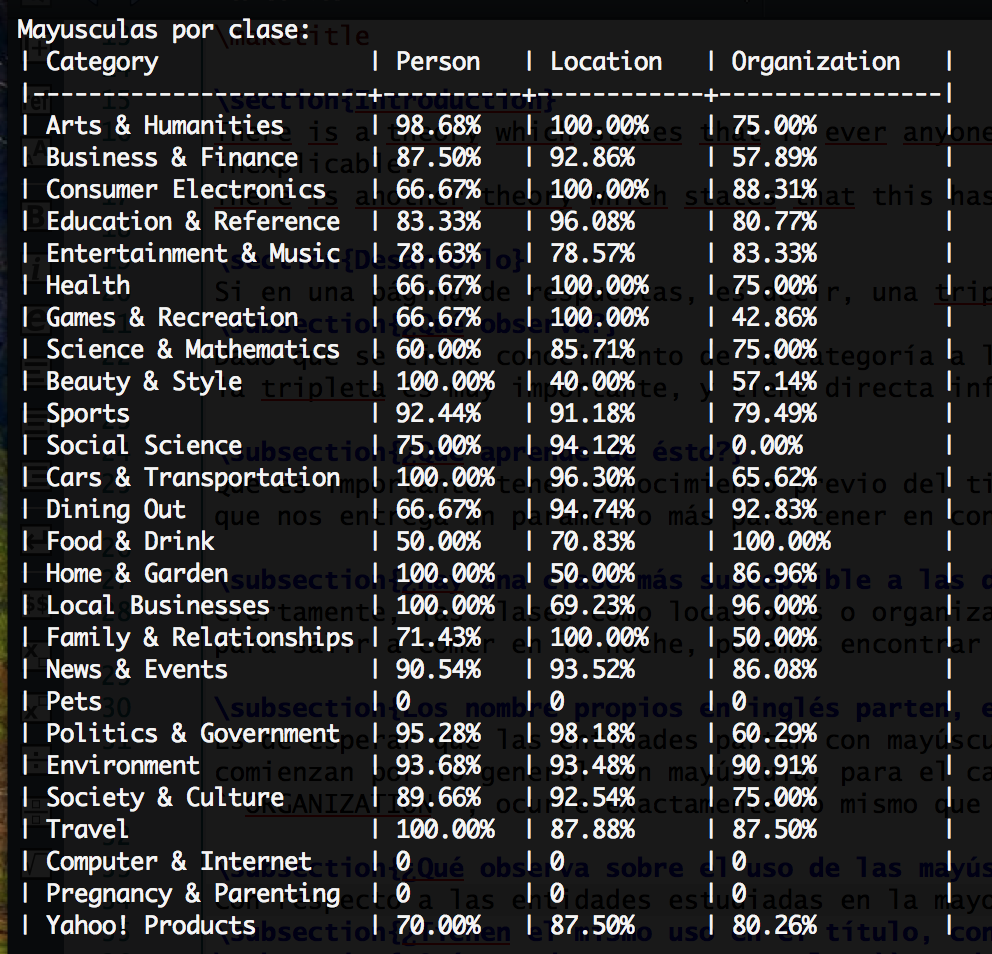
\includegraphics[scale=0.5]{figuras/mayusculas.png}
\caption{Mayúsculas por clase}
\label{fig:mayusculas}
\end{figure}

En la Figura~\ref{fig:mayusculas}, se aprecian las cantidades en porcentaje del uso de mayúsculas en los name entities obtenidos mediante el etiquetado manual, si bien hay categorías que tienen un porcentaje de cero, esto es debido a que el uso en esas categorías no es tan relevante para el tipo de tripleta que se está presentando. ¿Tienen el mismo uso en el título, contenido y respuestas? Si, esto se aprecia con mayor claridad en preguntas que tienen relación con persona, lugares y organizaciones, puesto que la mayoría de éstas se escriben con mayúscula inicial.

\subsection{¿Qué puede corroborar acerca del uso de la mayúscula y los ``tokens''?}
En este caso, nos sirve de ayuda para poder discriminar un token de un name entity manera más fácil, puesto que en las tres clases utilizadas para etiquetar un patrón común es el uso de mayúsculas al inicio de cada palabra, y desde luego al ser estás nombres propios.

\subsection{De las palabras que comienzan con mayúsculas ¿cuántas fueron reconocidas como ``named entities'' y cuántas como ``tokens''?}
En la Figura~\ref{fig:cuenta}, se observa la cuenta de la cantidad de palabras que son iniciadas con mayúsculas para cada ``name entity" reconocido, a su vez se presentan las palabras que no comienzan con mayúsculas, representando parte importante de los datos como ``tokens", también se observa la cuenta de cuantos ``Tokens" comienzan con mayúscula.
\begin{figure}[h!]
\centering
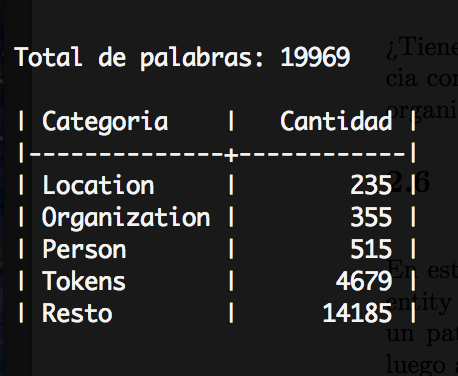
\includegraphics[scale=0.5]{figuras/mayus_word_token.png}
\caption{Cuenta de palabras iniciadas con mayúscula}
\label{fig:cuenta}
\end{figure}


\section{Pregunta 3}
\subsection{¿Cuántas de las palabras que fueron sugeridas en una de las tres clases de ``named entity'' y no fueron elegidas por ud. como tal fueron confusiones producto de errores ortográficos?}
Para este caso ningún ``named entity'' fue seleccionado por tener una discrepancia por faltas ortográficas, más bien los ``named entity'' que fueron sugeridos erradamente, fueron sugeridos mal por estar en un contexto errado.

\subsection{¿Qué puede concluir de aquello?}
Las sugerencias son muy útiles al momento de tener que determinar la pertenencia de una palabra a una clase determinada. Aportan mayor información al contexto, lo que permite una clasificación manual más rápida y segura.


\section{Pregunta 4}
\subsection{¿Qué sucede con las estructuras como tablas y listas? ¿Facilitan o dificultan la etiquetación?}
Facilitan mucho el etiquetado, ya que por lo general estas contienen a los ``named entity'', y su vez, estos tienen directa relación con la pregunta realizada.

\subsection{¿Qué sucede cuando la respuesta es la entidad?}
En este caso depende mucho de qué tan bien explicada esté la pregunta, ya que si no se explica bien el contexto, es muy difícil derivar una asociación coherente con la entidad.

\subsection{¿En este último caso se obtiene una buena o mala identificación? Ejemplifique. En estos casos ¿Las sugerencias son o no un aporte?}
Por lo general las sugerencias son un gran aporte ya que nos dan un indicio de que criterio utilizar al momento de etiquetar una entidad.


\section{Pregunta 5}
\subsection{Utilice MontyLingua para hacer un análisis morfológico y sintáctico de las palabras en las tripletas. ¿Qué observa?} 
En general las entidades no cambian su forma, los cambios más notorios son en aquellas entidades que podrían representar un plural, en este caso MontyLingua las lleva a su forma singular, lo cual en cierto sentido no alteraría el objetivo de la entidad. Por otra parte muchos token son eliminados ya que no representan mayor valor sintáctico dentro del conjunto de palabras que forman una tripleta.

\subsection{¿Las palabras que ud. etiqueto como entidades son susceptibles a ser mapeadas a una raíz o éstas no cambian?}
En su mayoría no cambian, salvo excepciones como se puede ver en la Figura~\ref{fig:lemmas}.
\begin{figure}[h!]
\centering
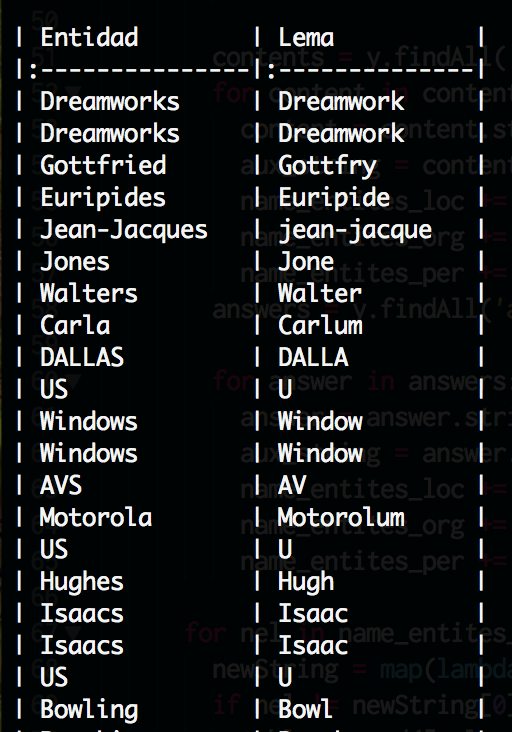
\includegraphics[scale=0.5]{figuras/lemmas.png}
\caption{Entidades lematizadas}
\label{fig:lemmas}
\end{figure}

\subsection{¿Hay una clase más afectada?}
En la Figura~\ref{fig:cambios} se puede ver como la clase ``organization'' es la que sufre mayores cambios con el uso de MontyLingua.
\begin{figure}[h!]
\centering
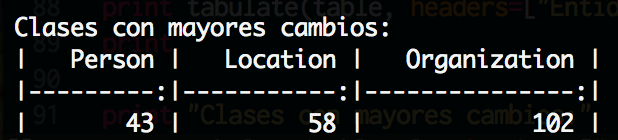
\includegraphics[scale=0.5]{figuras/cambios.png}
\caption{Entidades con cambios}
\label{fig:cambios}
\end{figure}
\subsection{¿Qué sucede con los tokens? En cuanto a las categorías sintáctica, ¿Cuál es la distribución en el conjunto de datos?}
Como se puede ver en la Figura~\ref{fig:sint_cat} las categorías sintácticas más relevantes dentro de los ``tokens'' es la clase NN, que representa a los sustantivos, y esto nos indica que están mayormente presentes en el texto que estamos analizando.
\begin{figure}[h!]
\centering
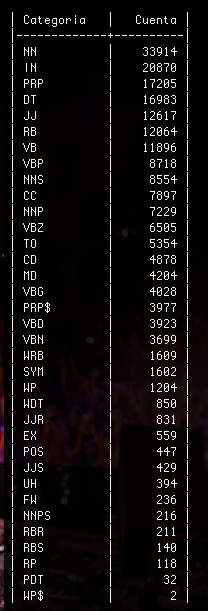
\includegraphics[scale=0.5]{figuras/sint_cat.png}
\caption{Entidades con cambios}
\label{fig:sint_cat}
\end{figure}

\newpage
\subsection{¿Cuáles son las cinco clases sintácticas más prominentes en cada una de las 26 categorías?} 
Esto se puede ver desde la Figura~\ref{fig:cat1} hasta la Figura~\ref{fig:cat26}.
\begin{figure}[h!]
\centering
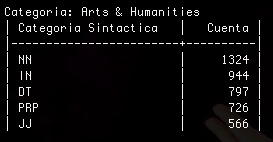
\includegraphics[scale=0.5]{figuras/cat1.png}
\caption{Arts \& Humanities}
\label{fig:cat1}
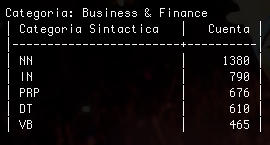
\includegraphics[scale=0.5]{figuras/cat2.png}
\caption{Bussiness \& Finance}
\label{fig:cat2}
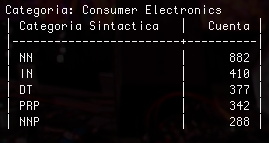
\includegraphics[scale=0.5]{figuras/cat3.png}
\caption{Consumer Electronics}
\label{fig:cat3}
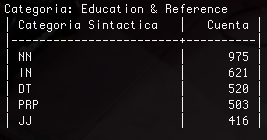
\includegraphics[scale=0.5]{figuras/cat4.png}
\caption{Education \& Reference}
\label{fig:cat4}
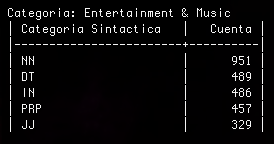
\includegraphics[scale=0.5]{figuras/cat5.png}
\caption{Entertainment \& Music}
\label{fig:cat5}
\end{figure}

\newpage
\begin{figure}
\centering
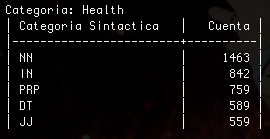
\includegraphics[scale=0.5]{figuras/cat6.png}
\caption{Healh}
\label{fig:cat6}
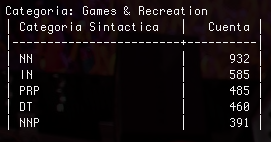
\includegraphics[scale=0.5]{figuras/cat7.png}
\caption{Games \& Recreation}
\label{fig:cat7}
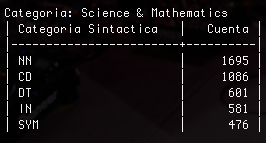
\includegraphics[scale=0.5]{figuras/cat8.png}
\caption{Science \& Mathematics}
\label{fig:cat8}
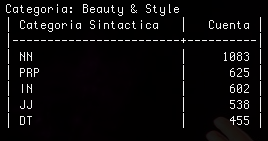
\includegraphics[scale=0.5]{figuras/cat9.png}
\caption{Beauty \& Style}
\label{fig:cat9}
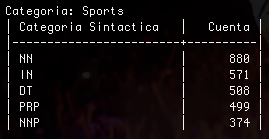
\includegraphics[scale=0.5]{figuras/cat10.png}
\caption{Sports}
\label{fig:cat10}
\end{figure}

\newpage
\begin{figure}
\centering
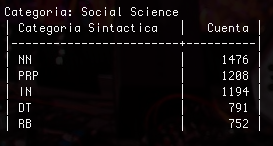
\includegraphics[scale=0.5]{figuras/cat11.png}
\caption{Social Science}
\label{fig:cat11}
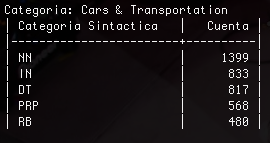
\includegraphics[scale=0.5]{figuras/cat12.png}
\caption{Cars \& Transportation}
\label{fig:cat12}
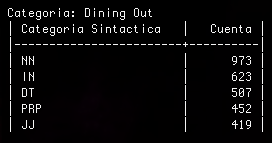
\includegraphics[scale=0.5]{figuras/cat13.png}
\caption{Dining Out}
\label{fig:cat13}
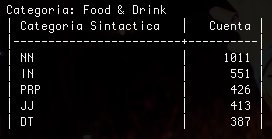
\includegraphics[scale=0.5]{figuras/cat14.png}
\caption{Food \& Drink}
\label{fig:cat14}
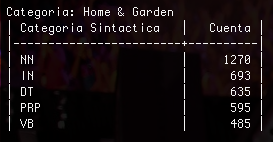
\includegraphics[scale=0.5]{figuras/cat15.png}
\caption{Home \& Garden}
\label{fig:cat15}
\end{figure}

\newpage
\begin{figure}
\centering
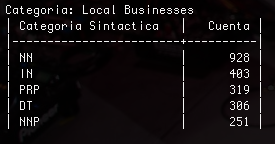
\includegraphics[scale=0.5]{figuras/cat16.png}
\caption{Local Businesses}
\label{fig:cat16}
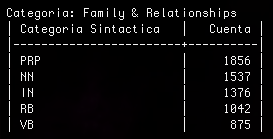
\includegraphics[scale=0.5]{figuras/cat17.png}
\caption{Family \& Relationships}
\label{fig:cat17}
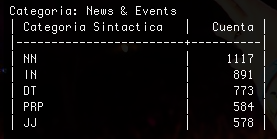
\includegraphics[scale=0.5]{figuras/cat18.png}
\caption{News \& Events}
\label{fig:cat18}
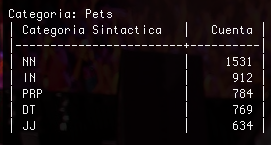
\includegraphics[scale=0.5]{figuras/cat19.png}
\caption{Pets}
\label{fig:cat19}
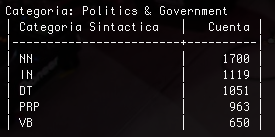
\includegraphics[scale=0.5]{figuras/cat20.png}
\caption{Politics \& Government}
\label{fig:cat20}
\end{figure}

\newpage
\begin{figure}
\centering
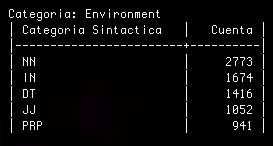
\includegraphics[scale=0.5]{figuras/cat21.png}
\caption{Environment}
\label{fig:cat21}
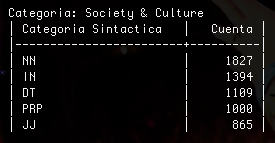
\includegraphics[scale=0.5]{figuras/cat22.png}
\caption{Society \& Culture}
\label{fig:cat22}
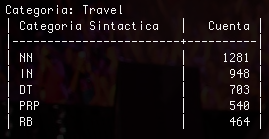
\includegraphics[scale=0.5]{figuras/cat23.png}
\caption{Travel}
\label{fig:cat23}
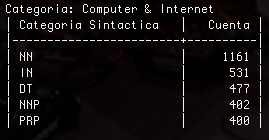
\includegraphics[scale=0.5]{figuras/cat24.png}
\caption{Computer \& Internet}
\label{fig:cat24}
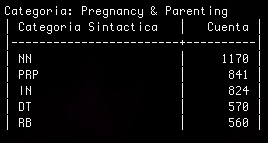
\includegraphics[scale=0.5]{figuras/cat25.png}
\caption{Pregnancy \& Parenting}
\label{fig:cat25}
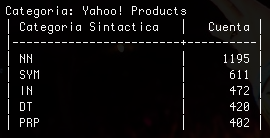
\includegraphics[scale=0.5]{figuras/cat26.png}
\caption{Yahoo! Products}
\label{fig:cat26}
\end{figure}

\newpage
\subsection{¿Cuál(es) es la categoría sintáctica más frecuente entre las palabras que etiqueto manualmente como ``named entity''?}
En la Figura~\ref{fig:pregunta5d} se puede ver que la categoría sintáctica NNP es la más común dentro de los ``named entity'' clasificados.
\begin{figure}[h!]
\centering
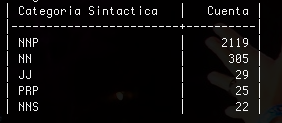
\includegraphics[scale=0.5]{figuras/pregunta5d.png}
\caption{Categoría sintáctica para ``named entity''}
\label{fig:pregunta5d}
\end{figure}


\section{Pregunta 6}
\subsection{Antes de una ``named entity'': ¿Cuál es la clase sintáctica más común?, y después de una ``named entity'' ¿Qué sucede?}
La Figura~\ref{fig:pregunta6}, muestra el conteo de las clases sintácticas que se detectan antes de un ``named entity''. Se puede apreciar como las clases sintácticas varían de acuerdo a si están antes o después de una ``named entity'', esto debido a la composición del texto, esto implica que algunas clases sintácticas aparecerían más que el resto.
\begin{figure}[h!]
\centering
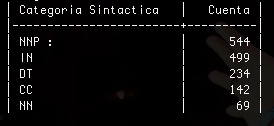
\includegraphics[scale=0.6]{figuras/pregunta6.png}
\caption{Clases sintácticas antes.}
\label{fig:pregunta6}
\end{figure}
\begin{figure}[h!]
\centering
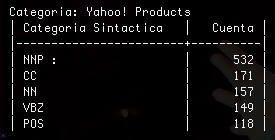
\includegraphics[scale=0.6]{figuras/pregunta6b.png}
\caption{Clases sintácticas después.}
\label{fig:pregunta6b}
\end{figure}
\subsection{¿Es para las tres clases de entidades lo mismo?}
En la Figura~\ref{fig:pregunta6c}, se muestran los resultados obtenidos para cada una de las entidades. Se puede ver que para cada una de las entidades hay clases sintácticas que predominan más que otras.
\begin{figure}[h!]
\centering
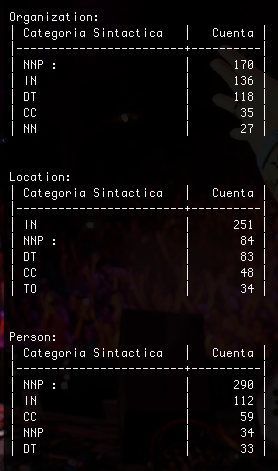
\includegraphics[scale=0.6]{figuras/pregunta6c.png}
\caption{Clases sintácticas por entidad}
\label{fig:pregunta6c}
\end{figure}


\section{Pregunta 7}
\subsection{Considerando un ejercicio binario 0/1, si una palabra es o no entidad. Calcule la accuracy, la precisión, el recall y el F-Score de la clase positiva (entidad). Para ésto, considere las sugerencias como respuesta automática y sus etiquetas manuales como la ``verdad absoluta''? También calcule la entropía del conjunto de datos considerando 0/1.}
La Figura~\ref{fig:pregunta7} muestra los resultados obtenidos, tanto para accuracy, precision, recall y F-Score, también se presentan los resultados para la Entropía de nuestro conjunto de datos. En este caso el accuracy está cerca del 70\% lo que nos indica que al rededor de un 70\% de las sugerencias fueron tomadas en cuenta al momento de etiquetar. 
\begin{figure}[h!]
\centering
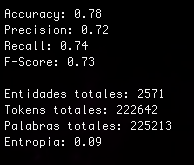
\includegraphics[scale=0.6]{figuras/pregunta7.png}
\caption{Calculo accuracy, precisión, recall, F-Score, Entropía.}
\label{fig:pregunta7}
\end{figure}

\newpage
\section{Pregunta 8}
\subsection{¿Qué observa para los ocho vectores?}
La Figura~\ref{fig:izquierdo}, muestra el resultado obtenido para los vectores de contexto izquierdo en el que podemos apreciar y de terminar que para este caso la palabra que más veces aparece antes de una de las clases es ``,'', por otra parte palabras como ``and'', ``the'', ``is'', ``to'', tienen alta frecuencia de aparición. En la Figura~\ref{fig:derecho} se muestran los resultados para las palabras con mayor aparición para cada clase. Se utilizó el carácter \#\makeatletter @\#\makeatletter @ se utilizó como cominzo y fin de linea.
\begin{figure}[h!]
\centering
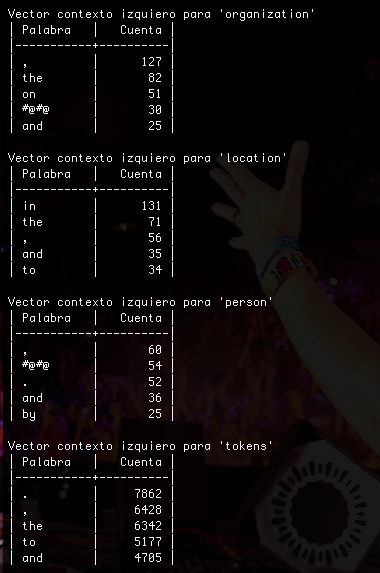
\includegraphics[scale=0.5]{figuras/izquierdo.png}
\caption{Vector de contexto izquierdo}
\label{fig:izquierdo}
\end{figure}
\begin{figure}[h!]
\centering
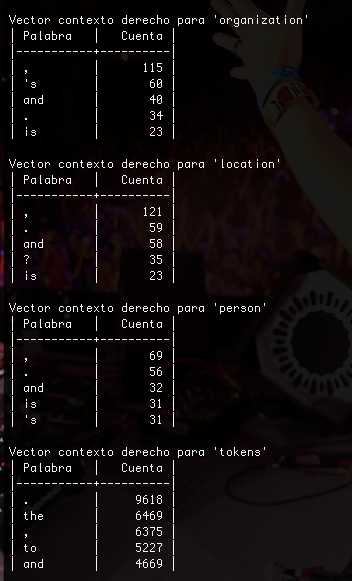
\includegraphics[scale=0.5]{figuras/derecho.png}
\caption{Vector de contexto derecho}
\label{fig:derecho}
\end{figure}

\newpage
\section{Conclusion}
\subsection{¿Qué indicadores hay en el texto que podría indicarme si una palabra es una ``named entity'' o no, si su clase respectiva?}
Como pudimos apreciar a través de este trabajo, existen muchos patrones los cuales no sirven para poder discriminar una ``named entity''. Por ejemplo, tenemos las categorías sintácticas que ya nos dan un indicio de lo que puede ser el contexto del texto que se está analizando o la presencia de algunos atributos importantes o la estructura de las respuesta, entregando así mayor información y facilitando la labor de etiquetado manual.

\subsection{¿Qué conclusiones cree que también se darían para el caso del idioma español?}
Posiblemente dependería mucho de las reglas que se utilicen para clasificar, como el español es un lenguaje rico en reglas quizás esto sea un punto a favor al momento de buscar la clasificación de las distintas entidades. Ahora bien, esto también puede llegar a ser un problema ya que si no se tiene conocimiento previo de estas reglas puede llegar a ser muy dificultoso clasificar.

\subsection{¿Qué características piensa ud. harían más fácil/difícil el reconocimiento de entidades en español?}
El genero, los tiempos verbales, las preposiciones, etc..., todas estás características hacen que el etiquetar en español sea algo más complicado, sobre todos para aquel que no domina el lenguaje o no tiene conocimiento completo de las reglas gramaticales con las que cuenta el español.

\subsection{¿Estaría un banco interesado en reconocer entidades? ¿En qué tipo de casos y para qué?}
Claramente que si, sería interesante el poder trabajar con las descripciones de los movimientos de las personas, con el objetivo de poder identificar que compran más o donde se va su dinero, así los bancos podrían separar a los grupos de personas y poder recomendarles productos acordes a su clase de gastos.

\subsection{¿Al gobierno le interesaría identificar entidades en alguna de sus base de datos?}
Como está de moda el emprender y el gobierno a hecho algunas plataformas digitales para poder facilitar eso, sería interesante poder trabajar en el ámbito del registro de patentes o marcas donde el poder identificar entidades como: una ``organización'' o la persona que esté a cargo del proyecto, puede ser de mucha ayuda para incluso poder clasificar a que rubro pertenece dicho emprendimiento y si hacer un mejor análisis de cuál es la tendencia real, al momento de crear una empresa.
\end{document}
